
\subsection*{Notação Sigma}


\begin{frame}[label=def_integral]
\frametitle{Notação Sigma }
\begin{small}
\noindent A notação sigma permite expressar uma soma com muitos termos em uma forma compacta.
$$\sum_{k=1}^na_k=a_1+a_2+a_3+\cdots+a_{n-1}+a_n$$

\begin{itemize}
\item O símbolo $\sum$ é chamado de somatório. Ele é a letra grega sigma maiúscula correspondente ao nosso S significa.

\item $k$ é o índice do somatório.

\item $a_k$ é o termo geral da soma.

\item 1 é o índice inferior e $n$ é o índice superior.

\end{itemize}

\end{small}

\end{frame}



\begin{frame}[label=def_integral]
\begin{exe}
\begin{enumerate}
\item $\dps\sum_{k=1}^4k^2=1+4+9+16=30$
\item $\dps\sum_{k=1}^5(-1)^k k=?$
\end{enumerate}
\end{exe}

\end{frame}

\subsection*{Somas de Riemann}

\begin{frame}[label=def_integral]
\frametitle{Partições de um intervalo }

\uncover<1->{Dado $[a,b]$ um intervalo fechado da reta,  o seguinte conjunto
\[P=\{x_0,x_1, \ldots, x_{n-1}, x_n\},\]
onde $a=x_0< x_1<\ldots < x_{n-1}< x_n=b$, é dito uma \dt{partição} de $[a,b]$.}
\medskip

\uncover<1->{Seja $\Delta x_i=(x_i-x_{i-1})$ o comprimento do intervalo $[x_{i-1},x_i]$ para todo $i=1,\ldots,n$. }

Um conjunto $\textcolor{blue}{\{c_1,c_2,\ldots,c_n\}}$, onde $\textcolor{blue}{c_i}\in[x_{i-1},x_i]$ é dito um \dt{pontilhamento} da partição $P$. Uma partição $P$ a qual escolhemos um pontilhamento  é dita uma \dt{partição pontilhada} e é denotada por $P^\ast$.
\medskip


%\uncover<1->{Definimos a \dt{norma } de uma partição $P$, denotada por $\|P\|$, como o maior dos $\Delta x_i$ com $i=1,\ldots,n$.}

\end{frame}


\begin{frame}[label=def_integral]
\frametitle{Somas de Riemann }

Seja $\textcolor{red}{f:[a,b]\to \R}$ uma função limitada e $P=\{x_0,x_1,\ldots,x_n\}$ uma partição qualquer de $[a,b]$.

\medskip


\uncover<1->{A soma
$$R(\textcolor{red}{f},P^\ast)=\sum_{i=1}^n\textcolor{red}{f}(\textcolor{blue}{c_i})\Delta x_i,$$
é dita uma \dt{soma de Riemann para f no intervalo [a,b]}.}
\medskip


\begin{center}
	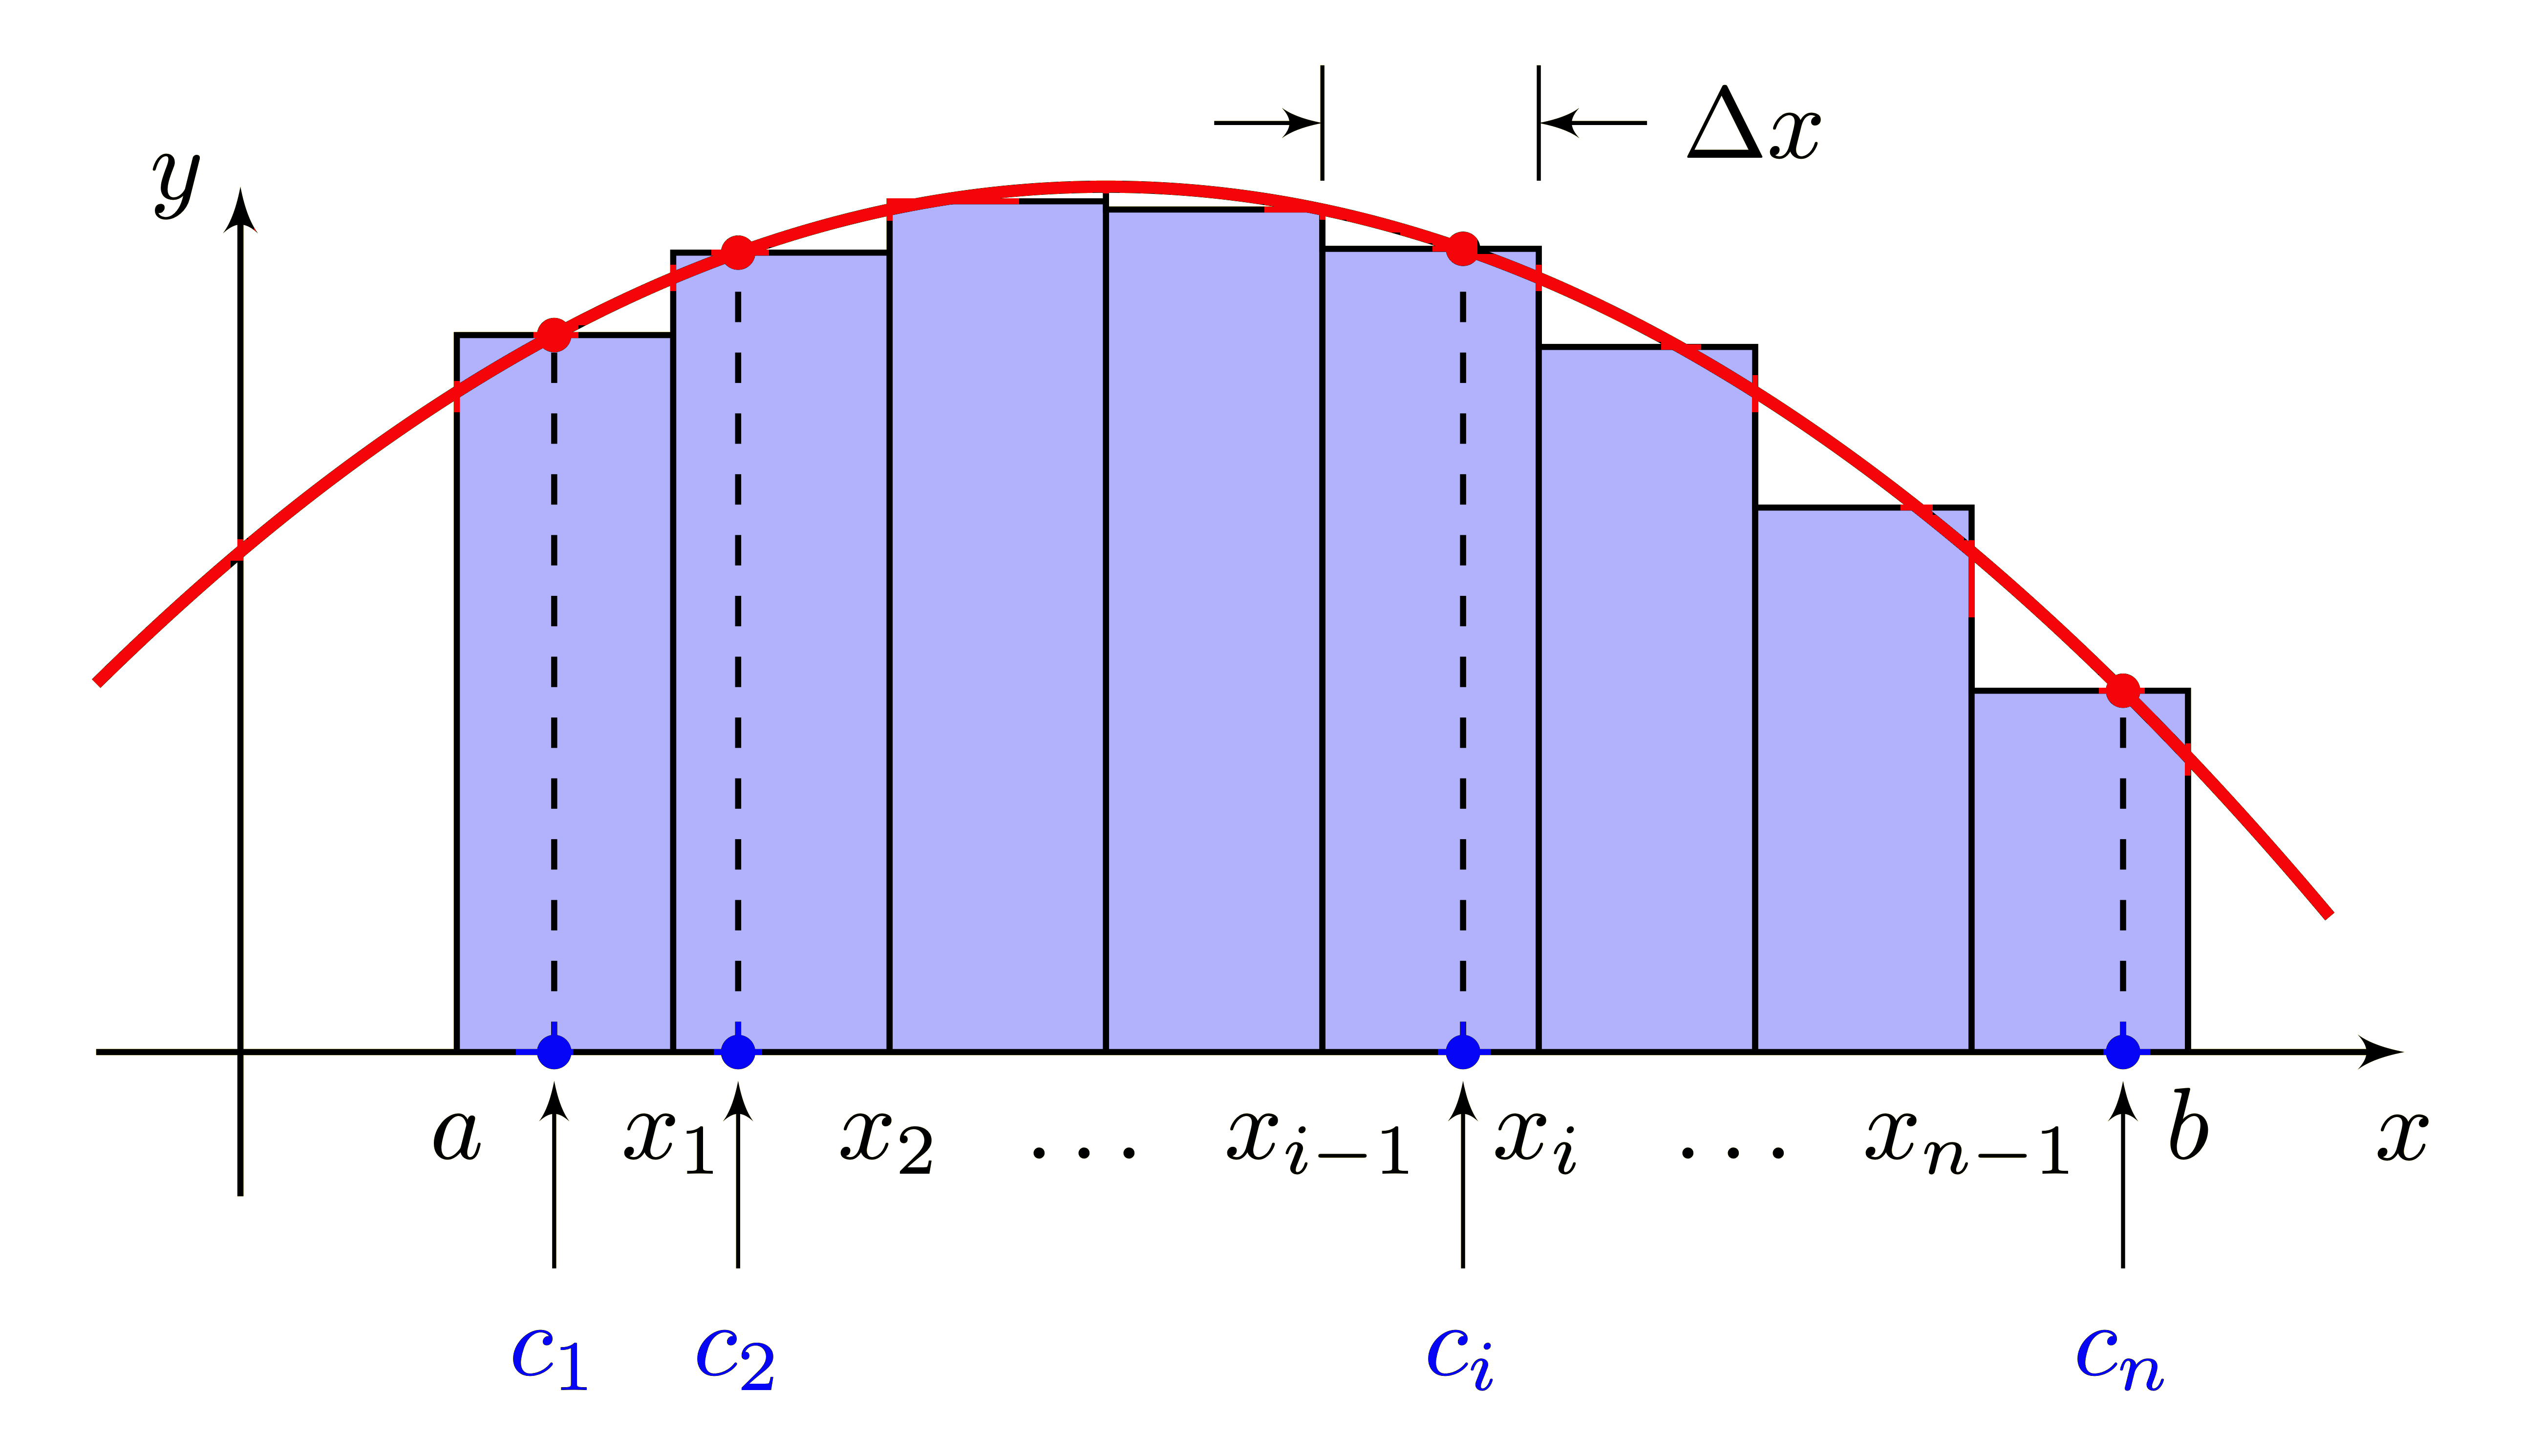
\includegraphics[scale=0.15]{capa3.png}
\end{center}


\end{frame}


\begin{frame}[label=def_integral]{Somas inferiores}
	\begin{itemize}
		\item $f:[a,b]\to \R$ contínua e $m_i=\dps\min_{[x_{i-1},x_i]}f(x)$
		
		\item $s(f,P)=\dps\sum_{i=1}^{n}m_i\Delta x_i$ \dt{somas inferiores } de $f$ em relação a $P$.
	\end{itemize}
	
%\uncover<1->{Dados uma função $f:[a,b]\to \R$ contínua e uma partição $P$  do intervalo $[a,b]$, definimos $m_i$ e $M_i$ como sendo o menor e o maior valor de $f(x)$ quando $x$ varia no intervalo $[x_{i-1},x_i]$, respectivamente.}
%\medskip
%
%\uncover<1->{Definimos ainda como $s(f,P)=\dps\sum_{i=1}^{n}m_i\Delta x_i$ e $S(f,P)=\dps\sum_{i=1}^{n}M_i\Delta x_i$ as \dt{somas inferiores } e \dt{somas superiores} de $f$ em relação à partição $P$, respectivamente.}
%\medskip

\begin{center}
	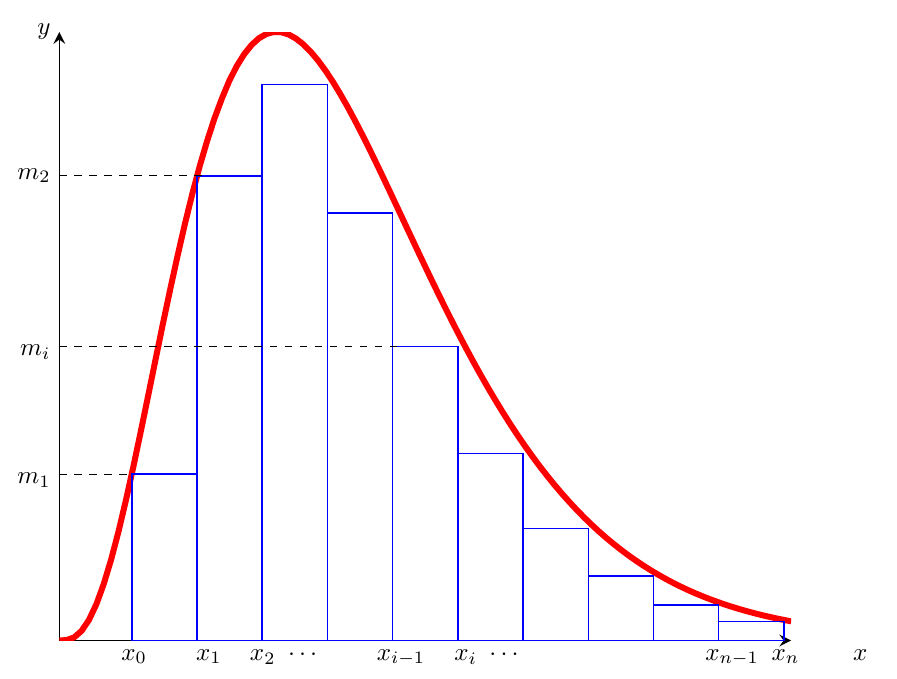
\includegraphics[scale=0.3]{som-inf.png}
\end{center}
\end{frame}


\begin{frame}[label=def_integral]{Somas Superiores}
	\begin{itemize}
		\item $f:[a,b]\to \R$ contínua e $M_i=\dps\max_{[x_{i-1},x_i]}f(x)$
		
		\item $S(f,P)=\dps\sum_{i=1}^{n}M_i\Delta x_i$ as \dt{somas superiores} de $f$ em relação a $P$.
	\end{itemize}
	\begin{center}
		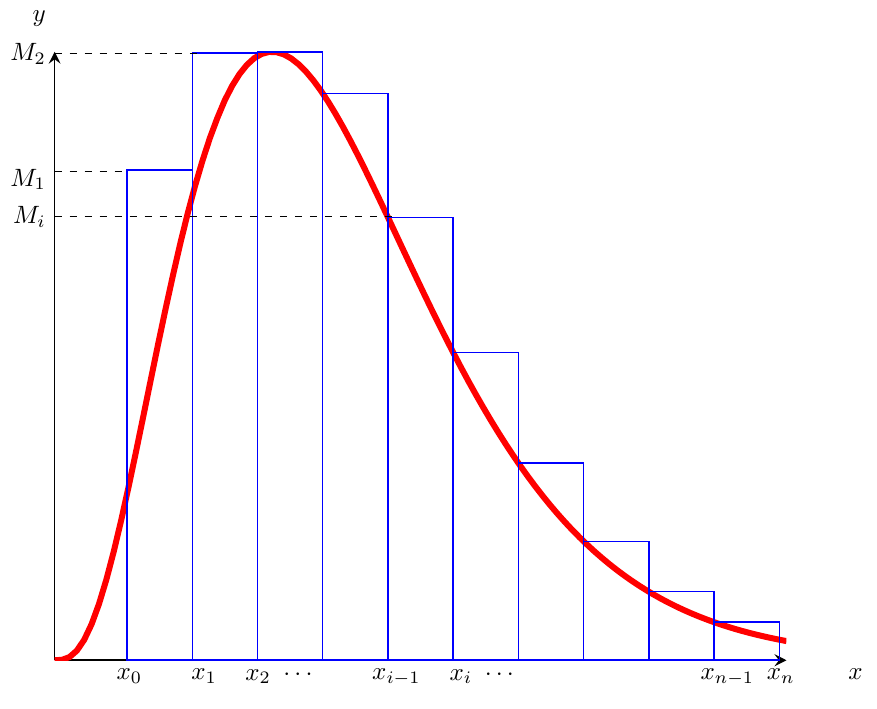
\includegraphics[scale=0.3]{som-sup.png}
	\end{center}
\end{frame}

\begin{frame}[label=def_integral]
\uncover<1->{\begin{exe}
 Encontre a área abaixo do gráfico de $f(x)=x^2$ quando $x\in[0,10]$.
\end{exe}}

\only<1>{
\begin{center}
	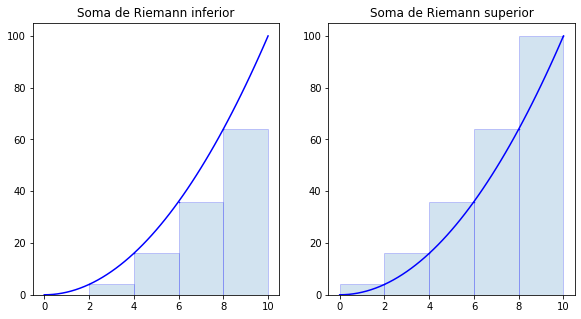
\includegraphics[scale=0.5]{int-rem1.png}
\end{center}

Partição com  {\color{red} 5 subintervalos} de mesmo comprimento.
\[s(f,P)=240\leq A\leq 440=S(f,P)\]}

\only<2>{
	\begin{center}
		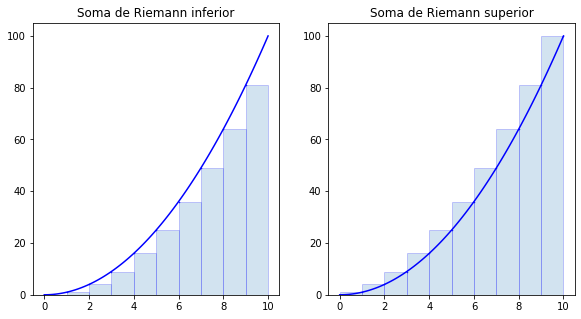
\includegraphics[scale=0.5]{int-rem2.png}
	\end{center}
	
	Partição com  {\color{red} 10 subintervalos} de mesmo comprimento.
	\[s(f,P)=285\leq A \leq 385=S(f,P)\]}

\only<3>{
	\begin{center}
		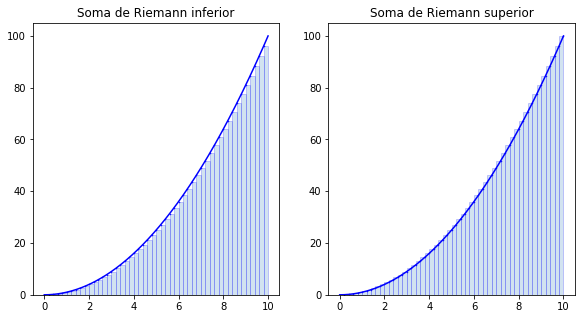
\includegraphics[scale=0.5]{int-rem3.png}
	\end{center}
	
	Partição com {\color{red} 50 subintervalos} de mesmo comprimento.
	\[s(f,P)=323\leq A \leq 343=S(f,P)\]}
\only<4>{
	\begin{center}
		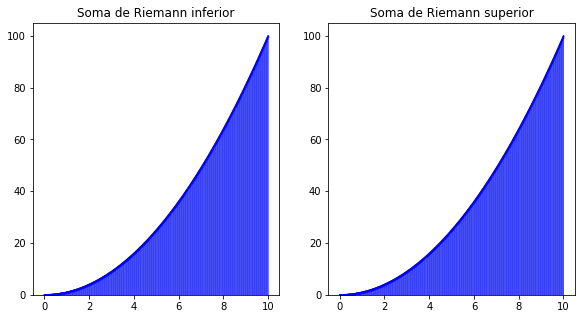
\includegraphics[scale=0.5]{int-rem4.png}
	\end{center}
	
	Partição com  {\color{red} 1000 subintervalos} de mesmo comprimento.
	\[s(f,P)=332.8335\leq A \leq  S(f,P)=333.8335\]}
%\end{small}

\end{frame}

\begin{frame}
\begin{casa}
Mostre que para $f(x)=x^2$, com $x\in[0,10]$, se $P$ é uma partição com $n$ subintervalos de mesmo comprimento, isto é, $\Delta x_i=10/n$, para todo $i=1,2,\ldots, n$, então
\[s(f,P)=\frac{1000}{n^3}\sum_{i=1}^{n}(i-1)^2\]
e
\[S(f,P)=\frac{1000}{n^3}\sum_{i=1}^{n}i^2.\]

Aplique o limite quando $n\to+\infty$ e conclua que a área abaixo do gráfico de $f$ é $\frac{1000}{3}$
\end{casa}
\end{frame}




\subsection*{Definição de Integral}
\begin{frame}[label=def_integral]


\uncover<1->{\begin{defin}Dizemos que uma função $f:[a,b]\to \R$ limitada é \dt{integrável em  $[a,b]$} quando existe um número real $I$ tal que 
$$\lim_{\|P\|\to 0}\sum_{i=1}^nf(c_i)\Delta x_i=I,$$
qualquer que seja a partição $P^\ast$. Em caso afirmativo dizemos que  $I$  é a \dt{integral} de $f$ em $[a,b]$ e o denotamos por $\int_a^bf(x)dx.$
\end{defin}}



\begin{center}
	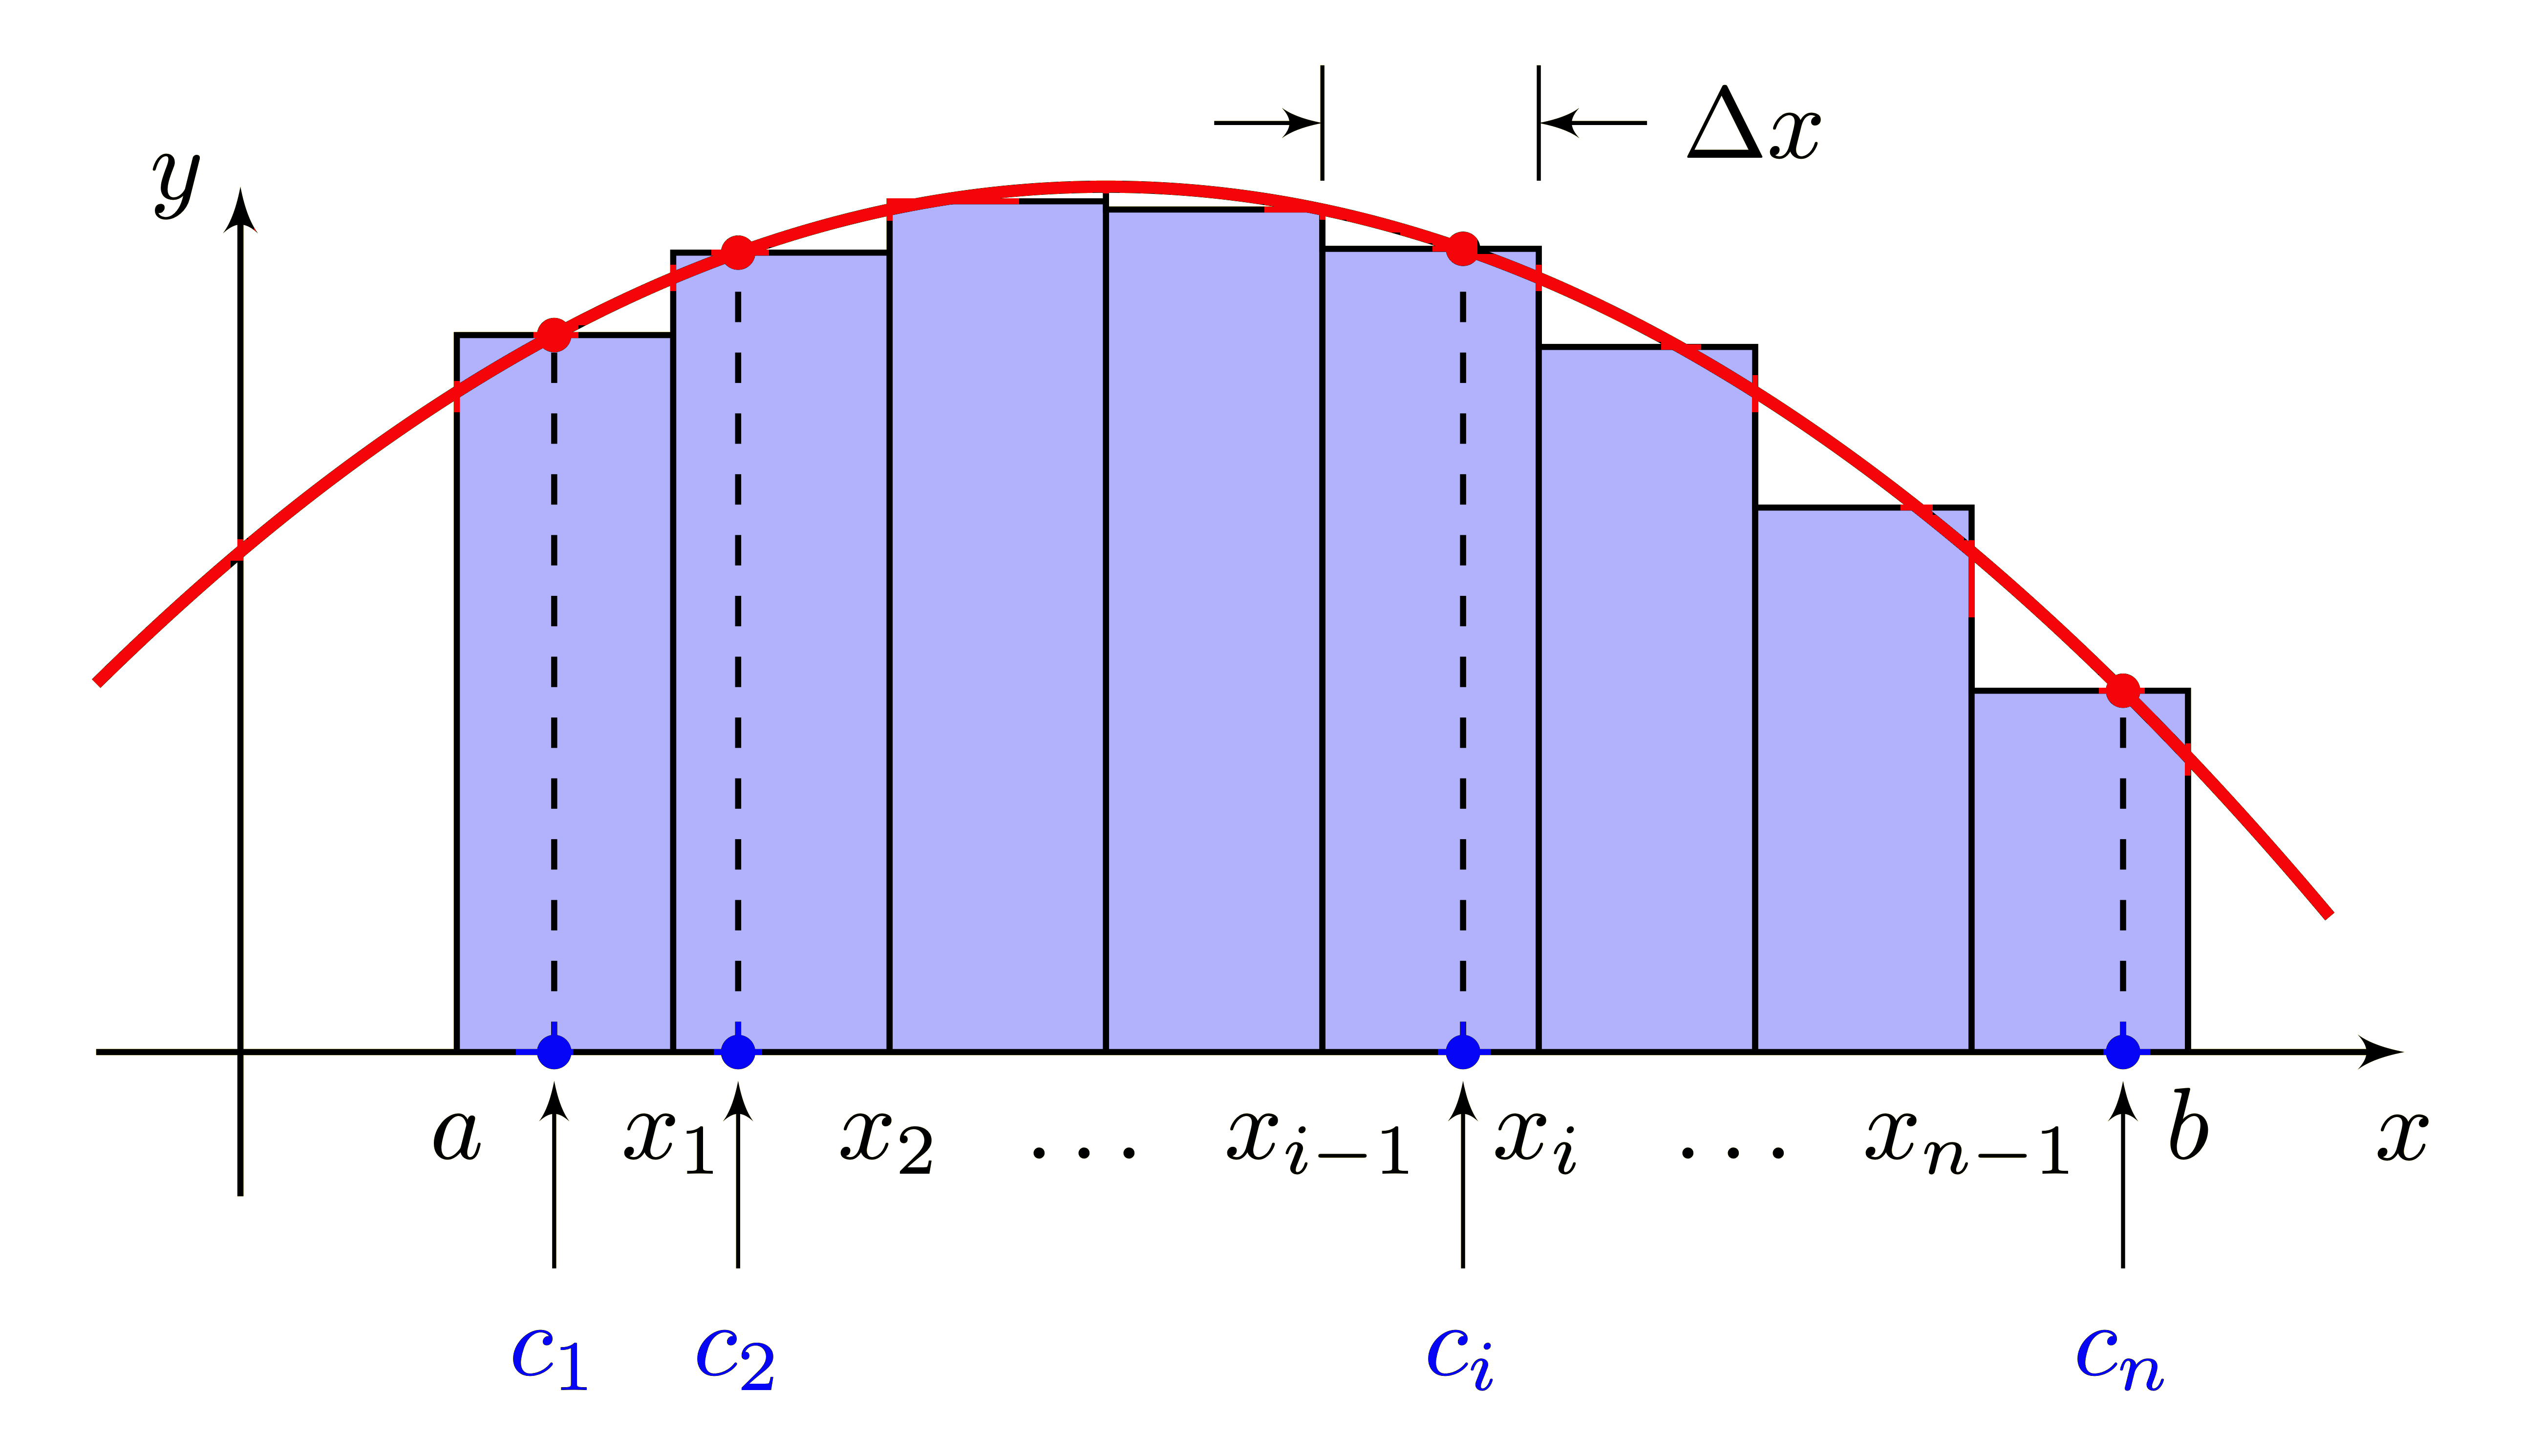
\includegraphics[scale=0.15]{capa3.png}
\end{center}
\end{frame}

\begin{frame}[label=def_integral]
\begin{block}{ }
O símbolo $\int$ de integral, que é um S alongado, foi introduzido por Leibniz em 1675. Leibniz não só tinha uma notável habilidade para construir notações; também criou termos como abscissa, ordenada, coordenada, eixo de coordenadas e função.  Quem primeiro usou a palavra ``integral" foi Jacob Bernoulli, em 1690.
\end{block}

\begin{block}{Área}
Pela construção,  quando $f(x)\geq 0$ para todo $x\in [a,b]$, vimos que a área abaixo do gráfico da função e acima do eixo $x$ é dada pela integral, isto é,
\[\text{Área}=\int_a^bf(x)\,dx\]
\end{block}
\end{frame}





\subsection*{Teorema Fundamental do Cálculo}




\begin{frame}[label=def_integral]
\frametitle{Teorema Fundamental do Cálculo }
\begin{small}


\uncover<1->{\begin{teo} Se $f:[a,b]\to \R$  é contínua e $F$ é uma primitiva de $f$, então
\begin{equation} \label{ident_TFC}\int_a^bf(x)dx=F(b)-F(a)\end{equation}
\end{teo}}

\uncover<1->{\begin{exe}
\begin{multicols}{2}
\begin{enumerate}
\item $\dps\int_0^1 x^2dx$
\item $\dps\int_0^1 x^3dx$
\item $\dps \int_a^b x^n dx$
\item $\dps\int_0^\pi \sen x\ dx$\\
\end{enumerate}
\end{multicols}
\end{exe}}



\end{small}
\end{frame}




\begin{frame}[label=def_integral]
\begin{small}

\uncover<1->{\begin{corol}\label{corol_TFC} Se $f:[a,b]\to \R$  é contínua, então
\begin{equation} 
\frac{d}{dt}\int_a^t f(x)dt=f(t), \forall t\in [a,b].
\end{equation}
\end{corol}}
\uncover<2->{
\begin{quote}
``O Teorema Fundamental do Cálculo é inquestionavelmente o mais importante do cálculo e realmente é um dos grandes feitos da mente humana. Antes de sua descoberta, desde os tempos de Eudóxio e Arquimedes até os de Galileu e Fermat, os problemas de encontrar áreas, volumes e comprimentos de curvas eram tão difíceis que somente um gênio poderia fazer frente ao desafio. Agora, porém, armado com o método sistemático que Leibniz e Newton configuraram a partir do Teorema Fundamental, veremos nos capítulos a seguir que esses problemas desafiadores são acessíveis para todos nós.''

\begin{flushright}
J. Stewart, Cálculo Vol. 1.
\end{flushright}
\end{quote}
 }

\end{small}
\end{frame}


\subsection*{Propriedades da Integral}
\begin{frame}[label=def_integral]
\frametitle{Propriedades da Integral }
\begin{teo} Se $f$ {\color{blue}for contínua em $[a,b]$}, ou tiver {\color{red}apenas um número finito de descontinuidades} do tipo saltos, então $f$ é integrável em $[a,b]$.
\end{teo}

\uncover<1->{Sejam $f$ e $g$ funções integráveis no intervalo $[a,b]$ e $k\in\R$ uma constante.

\begin{enumerate} 

\item $\dps \int_a^b k\ dx=k(b-a)$
\item $\dps \int_b^a f(x)dx:=-\int_a^b f(x)dx$ 
\item $\dps \int_a^a f(x)dx=0$
\end{enumerate} }

\end{frame}


\begin{frame}[label=def_integral]


\begin{enumerate}
\setcounter{enumi}{3}
\item $\dps \int_a^b kf(x)dx=k\int_a^b f(x)dx$
\item $\dps \int_a^b f(x)+g(x)dx=\int_a^b f(x)dx+\int_a^b g(x)dx$
\item $\dps \int_a^c f(x)dx+\int_c^b f(x)dx=\int_a^b f(x)dx$
\item  Se $f\leq g$, então $\dps \int_a^b f(x)dx\leq \int_a^b g(x)dx$
\end{enumerate}

\end{frame}




\begin{frame}[label=def_integral, fragile=singleslide]{Usando Python}
%\begin{small}
\begin{block}{ }
\begin{pyverbatim}
import sympy as sp

x = sp.symbols('x') #variável
f=sp.sin(x) #função

sp.integrate(f,(x,0,sp.pi)) #integral definida
\end{pyverbatim}
\end{block}
%\end{small}
\begin{pycode}
import sympy as sp

x = sp.symbols('x') #variável
f=sp.sin(x) #função
intf2=sp.integrate(f,(x,0,sp.pi)) #integral definida
intf=sp.integrate(f,x)
\end{pycode}

\[\dps \int_0^\pi \py{sp.latex(f)}\, dx=\py{sp.latex(intf)}\bigg\vert_{x=0}^{x=\pi}={\color{blue}\py{sp.latex(intf2)}}.\]
\end{frame}




\begin{frame}[label=def_integral]
	\begin{casa}
 Calcule as integrais
\begin{enumerate}[a]
	\item $\dps\int_1^3\frac{1}{x^2}\,dx$
	\item $\dps\int_1^2\frac{1}{x}\,dx$
	\item $\dps\int_{1}^{4} \frac{2x^
	3+x^3\sqrt{x}-1}{x^3}\,dx$
\end{enumerate}
	\end{casa}

\begin{casa}
Determine área da região limitada que está acima do eixo $x$ e abaixo do gráfico da função $y=x^3-x$.
\end{casa}
\end{frame}

